\section{Introduction}
\label{introductionsection}
\noindent \red{Over the last few years, we have observed a meteoric rise in the use and adoption of unmanned aerial vehicles (UAVs) and drones.} The first documented use of a drone for warfare occurred in  1849 when an unmanned balloon loaded with explosives attacked another town ~\cite{mckenna2016public}.
% After that, a generation of drones sparked in 1903 by the development of the fixed-wing aircraft. 
\textcolor{red}{
The development of fixed wing aircraft in 1903 sparked the development of a new generation of drones.}
% \todo{This line doesn't sound right}
The US army improved drones as weapons during the First World War, but those innovative drones were not deployed before the war ended in 1918. 
\red{World War II saw the first military use of drone as surveillance aircraft. The cold war between the east and the west further precipitated the development of drones as}.
% between many countries increased, enhancing the use of drones. 
many armed forces started using drones as a weapon, a reconnaissance tool, and a decoy. The progress of drone inspired both military and non-military companies to invest more in the field of drone research and development.

\textcolor{red}{Over the years,}
the drones saw exponential \textcolor{red}{development} for \textcolor{red}{regional} surveillance and supervision of remote construction projects. Rapid advancements in sensing, battery, and aeronautical technology, along with autonomous navigation methods and low-cost digital cameras have helped \textcolor{blue}{to} make the drone \textcolor{blue}{operations} more powerful, safer and \textcolor{blue}{reliable}\cite{liu2014review}. Since the early pioneering days, almost all types of active and passive sensors have been mounted on aerial systems, ranging from tethered to autonomous or manually operated \cite{sensing2015disasters, dong2013comprehensive}. With the help of these sensors, a drone can be deployed in many sectors, such as building inspection, rescue missions.
% , following an unidentified person, etc. 
In the present day, large number of organizations in different sectors are using drones to visually monitor the problems, 
find solutions, and even solve the problem based on the task\red{s}. Such systems are aimed at achieving more efficient service, inspection, and maintenance with minimal human intervention.

The drone-based \textcolor{blue}{monitoring} allows low-cost and frequent inspections \textcolor{blue}{with} high-resolution image analysis and limited human interference
% \st{, allowing for predictive maintenance} 
at reduced costs~\cite{morgenthal2014quality}. Lots of real-time problems exhibit recognizable visual characteristics that drones can \red{resolve} with RGB cameras~\cite{roy2013performance}. For example, cracks in the concrete 
% \st{of other} 
surfaces are visible by naked eyes. But it takes substantial manual effort to obtain damage information \red{around} \textcolor{blue}{large} scale areas.
\red{For example, taking pictures during manual inspection from a 40-50 feet height without costly safety gear poses serious risks of injury; maintaining precision while covering the whole are can also be challenging.}
% Additionally, \textcolor{blue}{frequent} manual inspection is not only challenging but also risky in some cases. Taking pictures \textcolor{blue}{from} a height \textcolor{blue}{of} 40 to 50 feet is dangerous because it may \textcolor{blue}{cause severe life threatening incidents.} 
% \st{be lethal if someone falls from that altitude} 
% Besides, 
% \textcolor{blue}{Maintaining precision and covering the whole area might not be possible with manual inspection.} 
% \st{important information might be left behind}.
\textcolor{blue}{However,} 
% \st{But in serval cases}, 
regular monitoring is necessary \textcolor{blue}{in several aspects of different domains, such as,} 
% \st{which can prevent several accidents, e.g.,} 
windmill turbine monitoring, building crack inspection, long bridge health investigation \textcolor{blue}{etc}. By 
% \st{supplying}
\textcolor{blue}{providing} 
% \st{experts with} 
automated feedback on 
% \st{highly}
\textcolor{blue}{most} likely 
% \st{locations}
\textcolor{blue}{region} of 
% \st{destruction}
\textcolor{blue}{interest where immediate action is needed}, we can significantly reduce the required man-hours \textcolor{blue}{for whole area inspection} and simultaneously increase the efficiency of \textcolor{blue}{resource usage}
% \st{manual detection, while reducing the human costs associated with the data inspection}. 
Besides \textcolor{blue}{of monitoring physical infrastructures,} 
% \st{building inspection}, 
drones can \textcolor{blue}{also} be used for \textcolor{blue}{other purposes, such as,} human 
% \st{suspectable} 
activity monitoring\textcolor{blue}{,}  
% \st{or}
rule-breaking vehicle tracking~\cite{ngo2019isir} \textcolor{blue}{etc}. Drones with 
% \st{other}
\textcolor{blue}{different} sensors can 
% \st{represent} 
\textcolor{blue}{provide variety of} other information \textcolor{blue}{of surroundings}, that can improve our daily livings in many ways~\cite{roy2015aarpa, pathak2015acoustic}. \textcolor{blue}{For an instance, hand-held or smartphone associated thermal cameras for detecting i}nsulation issues in 
% \st{built-up}
\textcolor{blue}{built-in} environments 
% \st{can be detected using a drone thermal camera which can save energy}
(i.e., ~\cite{khan2019detecting, khan2015demo, khan2020temporal}) \textcolor{blue}{ can be replaced by drone-based thermal camera for robust and scalable monitoring which can contribute to energy savings}. Common applications of drones in different sectors are shown in Fig~\ref{applicaitonfig}.


\begin{figure}[h!]
\centering
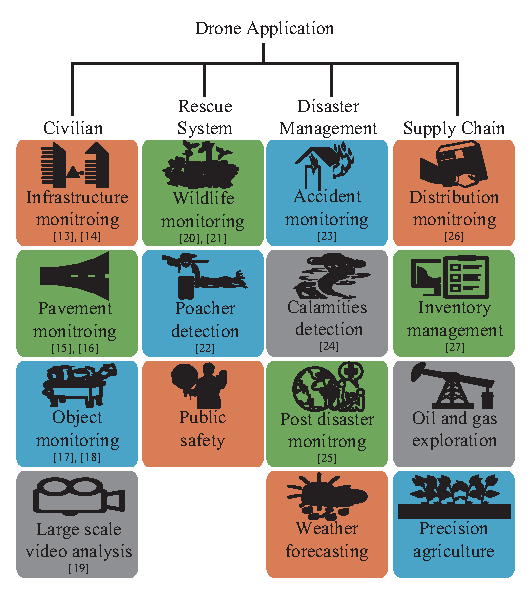
\includegraphics[width=.85\linewidth]{figure/applicaitonfig.eps}
\caption{Application of drone in different sector.}
\label{applicaitonfig}
\end{figure}
%\begin{table}[h]
\centering
\caption{Application of drones in different sector}
\begin{tabular}{|l|l|}
\hline
Category                             & \multicolumn{1}{c|}{Application}                                                                                             \\ \hline
\multirow{4}{*}{Civilian}            & Infrastructure crack detection~\cite{kucuksubasi2018transfer, kang2018autonomous}                                            \\ \cline{2-2} 
                                     & Road or pavement monitoring~\cite{wu2018coupling, fan2019real}                                                               \\ \cline{2-2} 
                                     & Object detection~\cite{li2017visual,saribas2019hybrid}                                                                       \\ \cline{2-2} 
                                     & Large scale video analysis~\cite{zhang2019dense}                                                                             \\ \hline
\multirow{2}{*}{Rescue system}       & Wildlife monitoring~\cite{mayer2019drones,brennan2019drones}                                                                 \\ \cline{2-2} 
                                     & Poacher detector~\cite{bondi2018spot}                                                                                        \\ \hline
\multirow{3}{*}{Disaster management} & \begin{tabular}[c]{@{}l@{}}Autonomous system able to explain\\ accident situations~\cite{garcia2018explainable}\end{tabular} \\ \cline{2-2} 
                                     & \begin{tabular}[c]{@{}l@{}}Calamities detector such as wildfire\\ with cameras~\cite{kyrkou2019deep}\end{tabular}            \\ \cline{2-2} 
                                     & Post-disaster assessment~\cite{tariq2018dronaid}                                                                             \\ \hline
\multirow{2}{*}{Supply Chain}        & \begin{tabular}[c]{@{}l@{}}Production and distribution monitoring\\ and prediction~\cite{apolo2020deep}\end{tabular}         \\ \cline{2-2} 
                                     & Inventory management~\cite{fernandez2019towards}                                                                             \\ \hline
\end{tabular}
\label{droneapplication}
\end{table}



\begin{comment}
% Please add the following required packages to your document preamble:
% \usepackage{multirow}
\begin{table}[]
\begin{tabular}{|l|l|}
\hline
Category                                                                    & Application                    \\ \hline
\multirow{4}{*}{Military}                                                   & Surveillance                   \\ \cline{2-2} 
                                                                            & Security                       \\ \cline{2-2} 
                                                                            & Air strike                     \\ \cline{2-2} 
                                                                            & Enemy tracking                 \\ \hline
\multirow{8}{*}{Commercial}                                                 & Shipping                       \\ \cline{2-2} 
                                                                            & Filming                        \\ \cline{2-2} 
                                                                            & Crop monitroing                \\ \cline{2-2} 
                                                                            & Irrigation                     \\ \cline{2-2} 
                                                                            & Architecture safety inspection \\ \cline{2-2} 
                                                                            & Mapping                        \\ \cline{2-2} 
                                                                            & Weather forecasting            \\ \cline{2-2} 
                                                                            & Supply chain                   \\ \hline
\multirow{5}{*}{\begin{tabular}[c]{@{}l@{}}Non-profit\\ usage\end{tabular}} & Traffic monitoring             \\ \cline{2-2} 
                                                                            & Rescue operation               \\ \cline{2-2} 
                                                                            & Disaster management            \\ \cline{2-2} 
                                                                            & Photography                    \\ \cline{2-2} 
                                                                            & Human health                   \\ \hline
\end{tabular}
\end{table}
\end{comment}

\textcolor{red}{Although} drones have a lot of useful applications, 
\textcolor{red}{there are still lingering challenges that hamper further adoption; }
% several challenges need to overcome
starting from the \textcolor{red}{limitations of the current} navigation systems to maintaining the privacy of \textcolor{red}{the} people. Therefore, in this paper, 
\textcolor{red}{in addition to discussing the application of drones,}
% we have discussed various applications of drones. 
% Besides, 
we have \textcolor{red}{articulated the} challenges, including \textcolor{red}{the} laws and legislation of different countries regarding drones \textcolor{red}{and} also \textcolor{red}{shed lights on the} the \textcolor{red}{recent} contribution of drones regarding tackling pandemics like COVID19. The organization of the paper is given below.

\subsection*{\textbf{Overview}}
In this article, we briefly discuss drone applications such as \textcolor{orange}{infrastructure monitoring~\cite{kucuksubasi2018transfer, kang2018autonomous}, pavement monitoring~\cite{wu2018coupling, fan2019real}, object monitoring~\cite{li2017visual, saribas2019hybrid}, large scale video analysis~\cite{zhang2019dense}, wildlife monitoring~\cite{mayer2019drones, brennan2019drones}, poacher detection~\cite{bondi2018spot}, public safety, accident monitoring~\cite{garcia2018explainable}, calamities detection~\cite{kyrkou2019deep}, post disaster monitoring~\cite{tariq2018dronaid}, weather forecasting, delivery package distribution monitoring\cite{apolo2020deep}, inventory management~\cite{fernandez2019towards}, oil and gas exploration, precision agriculture.}
%package delivery, site monitoring, disaster management, oil-gas exploration, weather forecasting, wildlife monitoring, precision agriculture~\cite{kucuksubasi2018transfer, kang2018autonomous, wu2018coupling, fan2019real, li2017visual,saribas2019hybrid, zhang2019dense, mayer2019drones,brennan2019drones, bondi2018spot,garcia2018explainable, kyrkou2019deep, tariq2018dronaid, apolo2020deep, fernandez2019towards}. 
\az{put the citations beside the application names}
Section~\ref{introductionsection} presents a short introduction, including a brief history of the drone's invention and evaluation story. Section~\ref{networkingsection} is divided into \textcolor{red}{three} subsections \textcolor{red}{where} we discuss \textcolor{red}{(i)} a few frameworks for autonomous drone navigation, \textcolor{red}{(ii)} how we can make the operation safer with obstacle avoidance technique, \textcolor{red}{(iii)} and we can handle drone data more efficiently. 
%In section~\ref{signalprocessingsection}, we have introduced research works that are aimed to handle drone data more efficiently. 
In section~\ref{applicationsection}, we mention machine learning-based drone applications that can improve our daily life. In section~\ref{datasetsection}, we \textcolor{red}{discuss on the drone related datasets}. In section~\ref{toolkitsection}, we analyze the hardware \textcolor{red}{components} of drones. In section~\ref{covid19section}, we describe the impact of COVID-19 on \textcolor{red}{sale and adoption figures pertaining to drones}. In section~\ref{challengesection}, \textcolor{orange}{we depict the challenges that researcher may face while working with drones} \textcolor{red}{and provide our concluding remarks in Section~\ref{conclusionsection}}
% Finally, we concluded our paper in section~\ref{conclusionsection}.
%\begin{table}[h]
\centering
\caption{Literature reviewed in this article}
\begin{tabular}{|c|l|}
\hline
Literature                                                                                                                                                                                                               & Brief description                                                                                 \\ \hline
\begin{tabular}[c]{@{}l@{}}\cite{tordesillas2019real}\\ \cite{tordesillas2019faster}\end{tabular}                                                                                                                        & Jump Point Search based autonomous navigation                                                     \\ \hline
\begin{tabular}[c]{@{}l@{}}\cite{padhy2018deep}\\ \cite{smolyanskiy2017toward}\end{tabular}                                                                                                                              & CNN based autonomous navigation                                                                   \\ \hline
\cite{jung2018perception}                                                                                                                                                                                                & \begin{tabular}[c]{@{}l@{}}Autonomous drone racing\\ Autonomous Drone Racing dataset\end{tabular} \\ \hline
\cite{garg2020enabling}                                                                                                                                                                                                  & Obstacle avoidance using Droppler effect                                                          \\ \hline
\cite{marcu2018safeuav}                                                                                                                                                                                                  & \begin{tabular}[c]{@{}l@{}}Safe landing plane detection\\ SafeUAV dataset\end{tabular}            \\ \hline
\cite{singla2019memory}                                                                                                                                                                                                  & Reinforcement learning based obstacle avoidance                                                   \\ \hline
\cite{kumar2018onboard}                                                                                                                                                                                                  & Data compression                                                                                  \\ \hline
\cite{milz2018aerial}                                                                                                                                                                                                    & Data augmentation with cGAN                                                                       \\ \hline
\cite{kouris2018learning}                                                                                                                                                                                                & Data augmentation with two-stream CNN                                                             \\ \hline
\begin{tabular}[c]{@{}l@{}}\cite{kucuksubasi2018transfer}\\ \cite{kang2018autonomous}\\ \cite{wu2018coupling}\\ \cite{fan2019real}\\ \cite{li2017visual}\\ \cite{saribas2019hybrid}\\ \cite{zhang2019dense}\end{tabular} & Deep learning based object detection and tracking                                                 \\ \hline
\begin{tabular}[c]{@{}l@{}}\cite{mayer2019drones}\\ \cite{brennan2019drones}\\ \cite{bondi2018spot}\end{tabular}                                                                                                         & Wildlife rescue system                                                                            \\ \hline
\cite{garcia2018explainable}                                                                                                                                                                                             & NLP for explaining incidence                                                                      \\ \hline
\cite{kyrkou2019deep}                                                                                                                                                                                                    & \begin{tabular}[c]{@{}l@{}}CNN based disaster detection\\ AIDAR dataset\end{tabular}              \\ \hline
\cite{tariq2018dronaid}                                                                                                                                                                                                  & Human rescue system                                                                               \\ \hline
\begin{tabular}[c]{@{}l@{}}\cite{apolo2020deep}\\ \cite{fernandez2019towards}\end{tabular}                                                                                                                               & Supply chain management                                                                           \\ \hline
\begin{tabular}[c]{@{}l@{}}\cite{zhu2018vision}\\ \cite{zhu2020vision}\end{tabular}                                                                                                                                      & Visdrone dataset                                                                                  \\ \hline
\cite{hsieh2017drone}                                                                                                                                                                                                    & CARPK dataset                                                                                     \\ \hline
\cite{du2018unmanned}                                                                                                                                                                                                    & UAVDT dataset                                                                                     \\ \hline
\cite{kyrkou2020emergencynet}                                                                                                                                                                                            & AIDAR dataset                                                                                     \\ \hline
\cite{jung2018perception}                                                                                                                                                                                                & Stanford Drone dataset                                                                            \\ \hline
\cite{gandhi2017learning}                                                                                                                                                                                                & Crash Itself datase                                                                               \\ \hline
\end{tabular}
\label{literature}
\end{table}
% \begin{figure}[h!]
% \centering
% 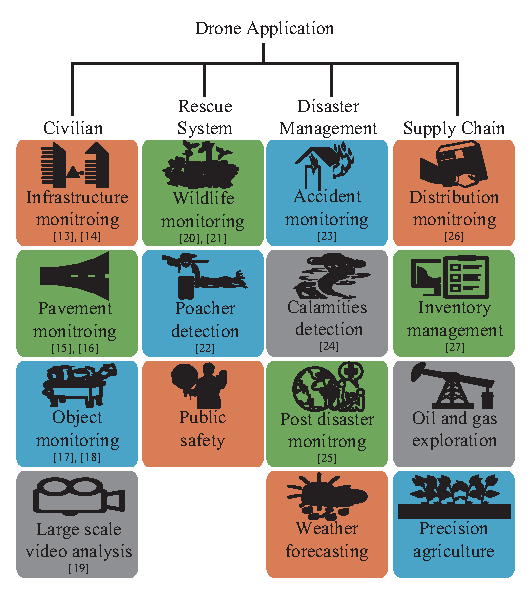
\includegraphics{figure/applicaitonfig.eps}
% \caption{Evaluation of commercial drone usage.}
% \label{applicaitonfig}
% \end{figure}